\chapter{System architecture} \label{chap:sys-arch}

In this chapter we will present the architecture that has been defined for the demonstration system.
During the course of this project's development phase, its architecture was continuously adapted as difficulties and possibilities emerged with the advancements made.

The following descriptions will reflect the final state of the proposed demonstrator, after several incremental iterations.
In relevant portions of this work, some comparisons will be made with the initial planned architecture to, not only demonstrate the iterative development process adopted but also to highlight some key aspects that benefited from this type of approach.

We will begin this chapter with an analysis of the requirements we should meet in order for the demonstrator to have certain characteristics, then present a detailed explanation of the actual proposed architecture, including the chosen hardware and software, finishing with a brief and non-exhaustive description of some conceptual experiments that could be possibly demonstrated on the proposed platform.

\section{Requirements analysis} \label{sec:requirements}

% Simplicity
% Low cost
% Robust (SW & HW)
% Modularity
% Visually/Physically based
% Control:
% - DCS
% - Local & Remote control
% - Velocity & Position

When considering the development of any practical demonstrator, some generic requirements should be taken into consideration due to the scope of such products.
These become even more relevant when the demonstrator is designed for educational purposes, as this is one such scenario.

The following subsections will delve into the main requirements of our project, explaining why they are being considered a requirement, how they were dealt with during development phase, what difficulties were encountered to meet such need and in which manner each requirement influenced the final system.

\subsection{Simplicity}

The most important characteristic every demonstrator should own is simplicity.
No matter how complex or extensive the concept might be, good demonstrators are conceptually simple.
Designs that focus solely on the concept at hand and leave out superfluous functionality tend to be more effective at conveying the main message.
Having the ability to further explore the concept beyond the initial scope of the demonstrator by extending its capabilities could be an advantage, but only when the implications of doing so do not hurt the initial simplicity.

In order to design a good demonstrator, simplicity should be the main focus in the early stages of research and concept design.
Contemplating different approaches based on simple concepts is crucial to ensure the end result is focused on the correct concept.
It is also very important to not allow underlying characteristics or design choices to outweigh the core concept.

\subsection{Low-cost} \label{sec:low-cost}

Demonstrators whose purpose is to serve as a first contact mechanism under an educational directive should be as low-cost as possible.
Accidents, bad practices or the simple lack of necessary knowledge can lead students and first-timers to, unintentionally, damage educational equipment.

Students tend to learn more easily when left to their own experiments, learning by themselves how things work and how to operate them. % TODO Cite something
For this to be possible, educational equipment should not impose limitations on the user freedom and, to meet such goal, low-cost is generically the best option.
Students must be able to experiment and learn without having to constantly worry about possible damage to expensive equipment.

\subsection{Modularity}

In addition to what is described in \autoref{sec:low-cost}, designing a system based on well defined modules is always a good thing.
Modularity helps divide the most complex systems into several, easier to handle, parts.
This characteristic also helps reduce costs, especially when considering the integration of pre-made modules, instead of developing new ones.

When there is possibility to design a product that reuses components and modules available on the market, production, maintenance and repairs become simpler and cost-effective.
With this approach, a damaged physical module can simply be replaced and software modules become easier to work with.
When developing software modules, one needs to pay close attention to the planned boundaries of each module, making sure their functionality is entirely self-contained.
This way, if we wish to replace a physical module we can also simply swap the respective software module with a new one, targetted at the new physical module.

\subsection{DCS based architecture}

With our aim being the influence of network cycle time on control applications, it's imperative for us to use an architecture that resembles a DCS system.
It only makes sense to evaluate such influence on systems where it is applicable, meaning, we must replicate a real world case where the usage of an RTE might actually influence the system performance.
With this in mind, we decided to replicate the concept of a networked servo drive controlled from a centralized processing unit, with the ability for the control loop to be closed either locally on the servo drive (the current typical scenario) or remotely on the processing unit.


\section{Proposed implementation}
Following the proposed architecture, presented in the previous chapter, we will now explain the actual implementation we performed to achieve our goals.
This section briefly presents the overall idea and proposed system architecture without going into details about specific choices.
Those explanations will be presented in later sections, as we will delve deeper into the implementation details, including product and technology choices, both in terms of hardware and software.

\subsection{Master node}
The master node of our system will be implemented in a generic desktop PC through the usage of an industrial programming platform.
This will enable us to program the behaviour of the master node as well as provide the necessary communication libraries to implement a master node for different RTE networks.
We will take advantage of the fact that most industrial programming platforms allow us to determine the RTE network's update period.
This will enable us to perform tests using different network cycle times.

Two programs will be developed for the master node:
\begin{enumerate}
	\item one to act as a simple set-point generator, sending the velocity or position set-points to the slave device through the RTE network;
	\item a second one to act as the motion controller, where the same set-points are used internally in a control algorithm that receives the plant feedback value and sends the plant output value through the RTE network.
\end{enumerate}

This implementation will allow us to perform the two practical experiments described in \autoref{sec:experiments}, enabling us to compare performance values acquired in both cases.

\subsection{Slave node}
The proposed slave implementation will be based on an embedded computing platform.
The embedded platform will be extended using some specialised boards that will broaden the functionality of the slave device as a whole.
These extension will provide easier access to the GPIO pins, direct interface with a motor through a specialised DC motor control board and Real-Time Ethernet connection using a dedicated board capable of off-loading the real-time processing of network packets from the embedded computing platform.

Additionally, in order to create a connection with the real world, we'll be using a DC motor paired with an incremental encoder.
This will allow data to be collected from a real world source, giving a more organic feeling to the process of running experiments with this system.

In terms of software, a control application will be developed for the slave device computing platform in order to provide the following functionality on the slave device:
\begin{itemize}
	\item Handle the receiving and sending of cyclic data through the RTE network by interfacing with the driver of the dedicated RTE network connection board. Such data will include set-point and feedback values;
	\item Handle the plant feedback signals, converting them into internal variables.;
	\item Handle the motor output signal by interfacing with the dedicated DC motor control board;
	\item Acquire and export performance data relating to the control of the DC motor speed and/or position;
	\item Provide an internal control algorithm to locally control the motor's speed and/or position;
\end{itemize}

Such software will be implemented in modules, and a general overview of how they interconnect with each other can be seen in a block diagram format in \autoref{fig:sw-architecture}.
The block names represent the actual names used for the different modules that were implemented.

\begin{figure}[htp]
	\centering
	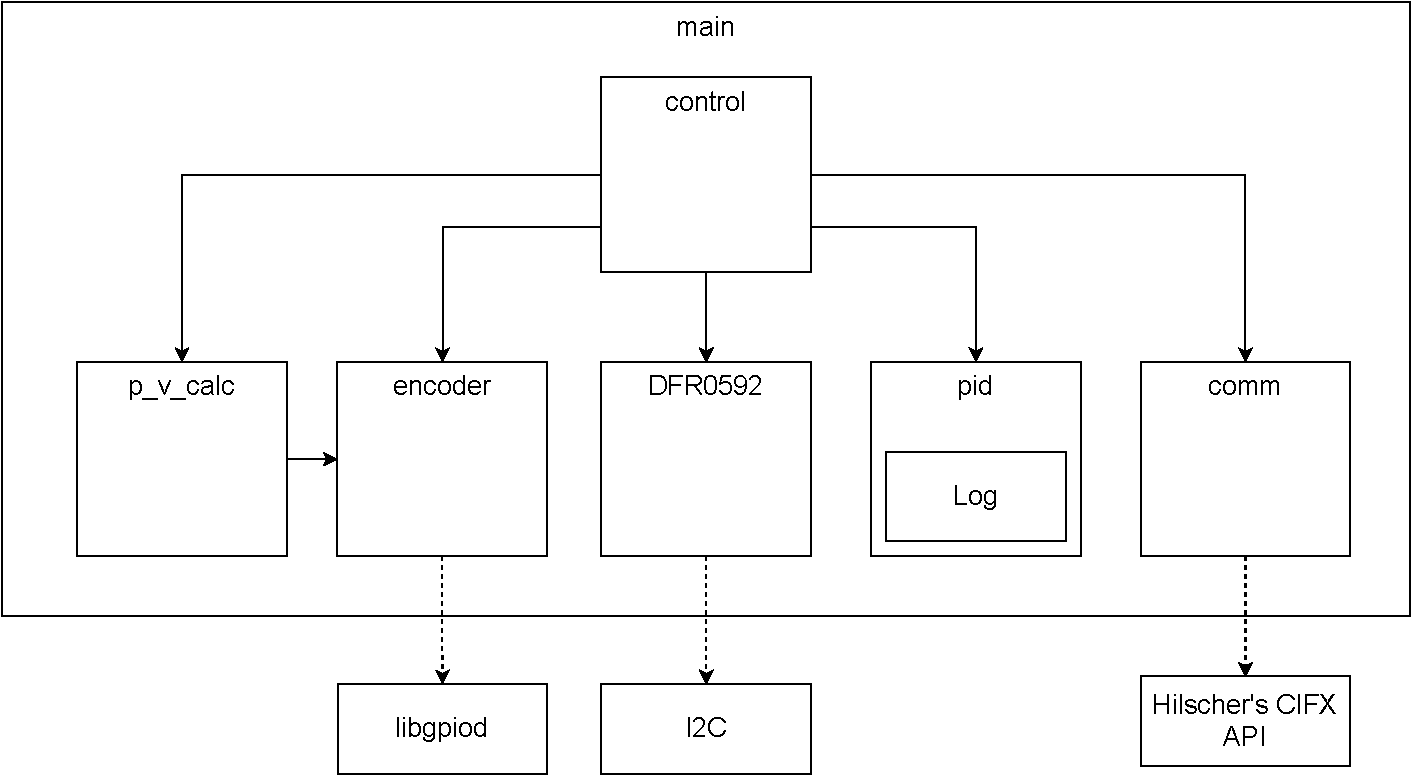
\includegraphics[width=0.8\linewidth]{sw-architecture.pdf}
	\caption{Slave device's software dependency graph}
	\label{fig:sw-architecture}
\end{figure}

The \verb|main| module will take care of initialising all data structures and sending the terminate commands when the user wishes to close the control application.
Configuration parameters can be passed as command-line arguments to the main module, which will be parsed and used during the run-time.
This module will serve as the entry point for the control application, where, after compilation, all modules will be integrated into a single executable.

The \verb|control| module will contain the function calls that determine the behaviour of the slave device during normal operation.
The run-time behaviour takes into consideration all parameters provided when launching the application.
It also takes care of moving data around between the other modules before calling functions that require some external data.
For example, the \verb|pid| module requires the set-point and plant feedback values, which are retrieved from the \verb|p_v_calc| module and \verb|comm| module, respectively.

The \verb|p_v_calc| module will be responsible for computing the motor velocity and position, based on an encoder counter.
Such counter is implemented on the \verb|encoder| module, which will convert the encoder signals onto a counter value.
In order to have access to the encoder signal, which will be connected to the GPIO header, we used the external library called \verb|libgpiod| to gain access to the GPIO pins.

The \verb|DFR0592| module is responsible for implementing functions to access and interface the DC motor control board.
All communication is done via I2C, which requires the usage of an external library.
In this particular implementation, we used the default Linux kernel I2C library.

The \verb|pid| module implements a discrete-time PID controller used for the local control of the motor's position or velocity.
Additionally, because all relevant data that describes the system performance is already contained in the PID data structure, we implemented the functionality of exporting such data on this module.

At last but not least, the \verb|comm| module will be responsible to make API calls to the RTE interface board driver, called \verb|CIFX|, in order to configure the RTE network and retrieve/send cyclic process data.
All the necessary steps to initialise, configure and manage the different RTE networks will already be implemented in the \verb|comm| module functions.


\section{Conceptual experiments} \label{sec:experiments}

With the proposed architecture in mind, which was described in section \ref{sec:proposed-arch}, we have envisioned a generalized conceptual experiment to fulfil the main goal of demonstrating the effects of the network cycle time influence in control applications.
We have defined it in a generic way so that variations and extensions to the base idea can easily be developed.
This way the demonstrator does not focus on a single possible experiment but on a set of experiments that share the same foundation.

The first and most basic conceptual experiment we considered involves predefining a velocity curve over a certain amount of time and executing it using both available control modes: the local control and the remote control.
Each of these will generate a trace log of velocity points (in this case) measured during execution.

Naturally, the definition of the movement curve can be randomly generated or taken from any real-world example, whatever interests the user the most.
Independently of which control mode is going to be be executed, the predefined movement curve is to be stored in the master node by whatever means, either hard-coded into the control program or by using some form of data storage and interpretation.
Because the master node's software implementation will be left to the end-user's responsability, so will be the generation or interpretation of reference values from the predefined movement curve.
The only thing to be taken into account is that depending on which control mode is being used at a certain time, the slave device expects to receive different types of data: for local control the slave device expects to receive the control reference values (directly taken from the predefined movement curve) and for remote control it expects to receive the duty-cycle percentage to be applied to the motor (the actual 'output' value of the control loop).

As we aim to provide the means to export the recorded command and feedback values as a CSV file, we can now import them into any data processing software and perform relevant operations between the two traces.
The most simple comparison possible, and possibly the most effective, is to generate a graph that includes the two datasets simultaneously, which will create a visual representation of the system's performance in both control cases, making any differences in their behaviour quickly perceivable.




\section{Summary} \label{sec:impl-summary}
This chapter focused almost exclusively on technical details of how the final solution was implemented.
Starting with the choice of hardware components, going through their assembly and then moving towards the complex and extensive software required to give the desired slave device all planned functionality.

Not only the good things have been explained but we have also expressed those we are aware could have been better implemented or designed.
Even though this project was developed during difficult times, especially from having been done entirely on a full-remote work basis, most of the things explained as weak spots were considered from the beginning.
Difficult times impose harder decisions and \emph{simplify} became the daily word of choice because, sometimes, \emph{less is much more}.
It's one thing to design simple systems, but it's a much harder thing to simplify complex systems and boil them down to their bare-bones.

